% ------------------------------------------------------------------------------------------- %
%                                         Metodologia                                         %
% ------------------------------------------------------------------------------------------- %
\chapter{Materiais e Métodos}\label{cap:materialemetodos}

\section{Materiais}\label{sec:materiais}

\subsection{Plataforma Lattes}\label{subsec:lattes}

A plataforma Lattes, concebida em agosto de 1999, representa a experiência do \gls{cnpq} na integração de bases de dados de currículos e de instituições da área de ciência e tecnologia em um único sistema de informações, padronizando em âmbito nacional o formato para coleta de informações curriculares e cuja importância atual se estende, não só às atividades do \gls{cnpq}, como também às ações de incentivo a outras instituições federais e estaduais \cite{Lattes}.

A plataforma também possui uma página web para busca textual dos currículos cadastrados em seu sistema bem como uma ferramenta para extração de dados de sua base denominado \textit{Lattes Extrator}, porém tal ferramenta só é disponibilizada às instituições, que devem efetuar cadastro e solicitar acesso à mesma.

Há a possibilidade de não se obter acesso à ferramenta do \textit{Lattes Extrator}, e caso este risco venha a se concretizar duas alternativas serão consideradas. A primeira é a extração dos dados de maneira indireta através de requisições \gls{http} feitas para a ferramenta pública de busca da própria plataforma Lattes no seguinte formato \textit{\url{https://buscatextual.cnpq.br/buscatextual/download.do?metodo=apresentar&idcnpq=IdLattes}}, onde \textbf{IdLattes} é o id público de cada cientista cadastrado e disponibilizado no portal da memória da plataforma \cite{CnpqMemoria}. Esta requisição tem como retorno um arquivo no formato \gls{xml} contendo as informações do cientista que serão salvas na base de dados da plataforma.

Caso a segunda opção também se mostre problemática, a plataforma permitirá então, que os dados de cientistas possam ser cadastrados assim como o de empresas, centralizando dessa forma todas as informações necessárias na base de dados deste projeto.

\subsection{PostgreSQL}\label{subsec:postgresql}

O PostgreSQL é um banco de dados relacional contributivo, ou seja, tem seu desenvolvimento em código aberto, o que garante mais liberdade no uso, além de permitir diferentes implementações de acordo com as necessidades, e ele utiliza a linguagem SQL como base \cite{Amazon}. Muitos dos contribuintes são voluntários, mas o projeto se sustenta com patrocínios de diversar empresas de todo o mundo. É um projeto da Universidade da Califórnia em Berkeley e tem mais de 35 anos de desenvolvimento ativo na plataforma central \cite{PostgreSQL}.

\subsection{Linguagem C{\#} {\&} .NET Framework}\label{subsec:csharp}

C{\#} é uma linguagem de programação, fortemente tipada e orientada a objetos desenvolvida pela Microsoft em julho de 2000 e sua sintaxe foi baseada no C++ porém contendo influências de outras linguagens como Java. A linguagem permite que desenvolvedores construam diversos tipos de aplicações de forma segura e robusta que são executadas sobre a plataforma .NET \cite{CSharp}.

.NET Framework é uma plataforma de desenvolvimento que possui um \gls{clr}, que gerencia a execução de código. Possui também uma \gls{bcl}, oferecendo um amplo leque de classes para a construção de aplicações. A Microsoft, sua desenvolvedora, modelou a ferramenta para uso multi-plataforma, porém a ferramenta funciona melhor com o sistema operacional Windows \cite{CSharpDevelopment}.

\subsection{Flutter {\&} Dart}\label{subsec:flutterdart}

Flutter é uma estrutura que tem seu desenvolvimento em código aberto, disponível pelo Google. Com apenas um código, é possível construir aplicativos em multi-plataformas (Android/iOS), utilizando componentes nativos de cada plataforma \cite{Flutter}. A estrutura utiliza a linguagem Dart, que é assíncrona e muito semelhante a linguagem JavaScript \cite{Dart}.

\subsection{Docker}\label{subsec:docker}

Docker é um motor de código aberto que automatiza a implementação de aplicações dentro de containers. Esta ferramenta torna possível a criação de aplicações mais portáteis, de fácil construção e colaboração, reduzindo o tempo em que um código escrito seja testado, implementado e utilizado \cite{TheDockerBook}.

\section{Métodos}\label{sec:metodo}

\subsection{Aplicação Mobile}\label{subsec:app}

O desenvolvimento da Aplicação foi Mobile, pela facilidade e praticidade dos usuários se conectarem de qualquer lugar, requerindo apenas acesso a internet. A aplicação utilizou Flutter {\&} Dart, o que possibilita uma compatibilidade com sistemas Android e iOS. O propósito do aplicativo, é fornecer uma interface clara para login, cadastro das demandas, e para cada demanda, notificar os cientistas aptos, para que consigam se candidatar à elas.

O principal objetivo, é o desenvolvimento para a plataforma Android, sabendo que a maioria das pessoas, no Brasil, utilizam esse sistema operacional \cite{StatCounter}. Além de, para a disponibilização em iOS, é necessário um equipamento do sistema operacional para compilar o aplicativo.

\subsection{API REST}\label{subsec:apirest}

Para atender a necessidade de comunicação entre a aplicação cliente e as ferramentas empregadas na construção desta plataforma escolheu-se desenvolver uma \gls{api} \gls{rest}. Este tipo de aplicação pode ser descrita como um conjunto de serviços web hospedados em um servidor que expõem um conjunto de funcionalidades e dados de forma pública com o intuito de facilitar as interações e troca de informação entre programas de computador \cite{RestApiBook}.

Uma das principais vantagens de se utilizar uma \gls{api} \gls{rest} é sua escalabilidade, pois a aplicação simplesmente atende à requisições realizadas através de protocolo \gls{http} sem distinguir o tipo ou a quantidade de clientes, separando assim as regras de negócio relacionadas a manipulação de dados, das regras da aplicação de interface de usuário.

Este tipo de aplicação também possui uma implementação relativamente rápida e simples, onde cada possível requisição necessária pode ser facilmente adicionada a um controlador que gerência o acesso e a resposta para cada uma. Os testes sobre a aplicação também são simples, pois utilizam protocolo \gls{http} e podem por muitas vezes serem testados utilizando apenas um navegador web.

\subsection{Integrações}\label{subsec:integrar}

Uma das atividades mais importantes é a integração entre as ferramentas, e uma relação básica entre elas pode ser vista na figura \ref{fig:diagrama}. A aplicação mobile realiza requisições \gls{http} baseado nas entradas do usuário e estas requisições são atendidas pela \gls{api}, hospedada em um servidor que se situará nos domínios da \gls{utfpr}, retornando uma resposta no formato \gls{json}.

A \gls{api} também é responsável pela consulta de dados cadastrados na base da plataforma bem como a persistência de informações na mesma. Com o acesso as informações contidas na plataforma Lattes de cada cientista a \gls{api} também realizará a tarefa de consultá-las sempre que necessário, como por exemplo no momento do cadastro de um cientista, explicado na seção \ref{subsec:cadastro}.

\begin{figure}[htb]
    \caption{Diagrama das integrações entre aplicações}
    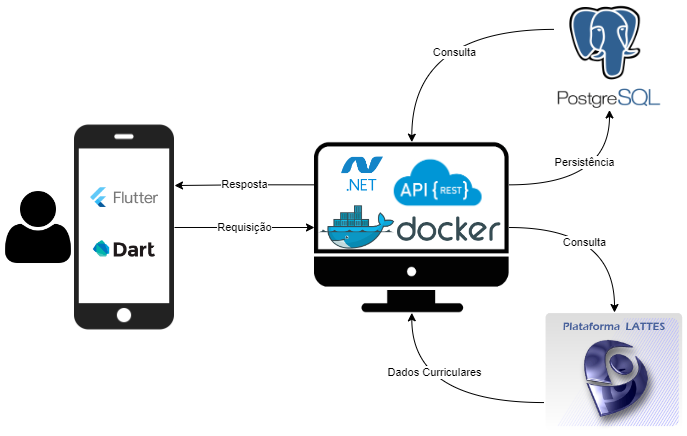
\includegraphics[width=0.8\textwidth]{DiagramaPlataforma}
    \fonte{Autoria Própria}
    \label{fig:diagrama}
\end{figure}

\subsection{Cadastro de Cientistas}\label{subsec:cadastro}

A inserção de usuários cientistas na plataforma poderá se dar de duas maneiras, a depender da possibilidade de se obter os dados relacionados da plataforma Lattes. Para o caso em que isto seja possível, no momento do cadastro, o usuário irá informar seu \textit{Id Lattes}, bem como uma senha. Utilizando o id informado, a plataforma irá então consultar na base do Lattes o email vinculado a esta informação e enviará para este email uma mensagem de confirmação, realizando assim a autenticação do cientista. Um problema óbvio surge deste método, a não existência de um email vinculado ao \textit{Id lattes} informado. Neste caso a plataforma irá então requerer que o usuário atualize esta informação ná sua pagina Lattes.

No caso da impossibilidade de se extrair dados da base do Lattes, no momento do cadastro de um cientista será requerido então que todas as informações necessárias para que o mesmo possa ser devidamente classificado dentro da plataforma sejam informadas. 

\subsection{Fluxo Proposto}\label{subsec:fluxo}

Quando uma empresa realizar o cadastro de uma demanda tecnológica e todas as informações necessárias para que essa demanda possa ser atendida tenham sido fornecidas, como por exemplo, área de atuação específica, tempo limite de entrega, orçamento, região de atuação e artefatos tecnológicos relevantes, esta demanda então será inserida na base de dados e uma notificação será enviada a todos os cientistas que cumpram as exigências impostas. 

Ao acessar a plataforma, um cientista poderá então visualizar a lista de demandas as quais está apto a atender, podendo assim confirmar sua intenção de atendê-lá. Ao fazê-lo, a empresa que gerou a demanda terá incluído na lista de possíveis parceiros o cientista, podendo assim iniciar as tratativas para a formação de uma parceria.

\begin{figure}[htb]
    \caption{Fluxo de uso}
    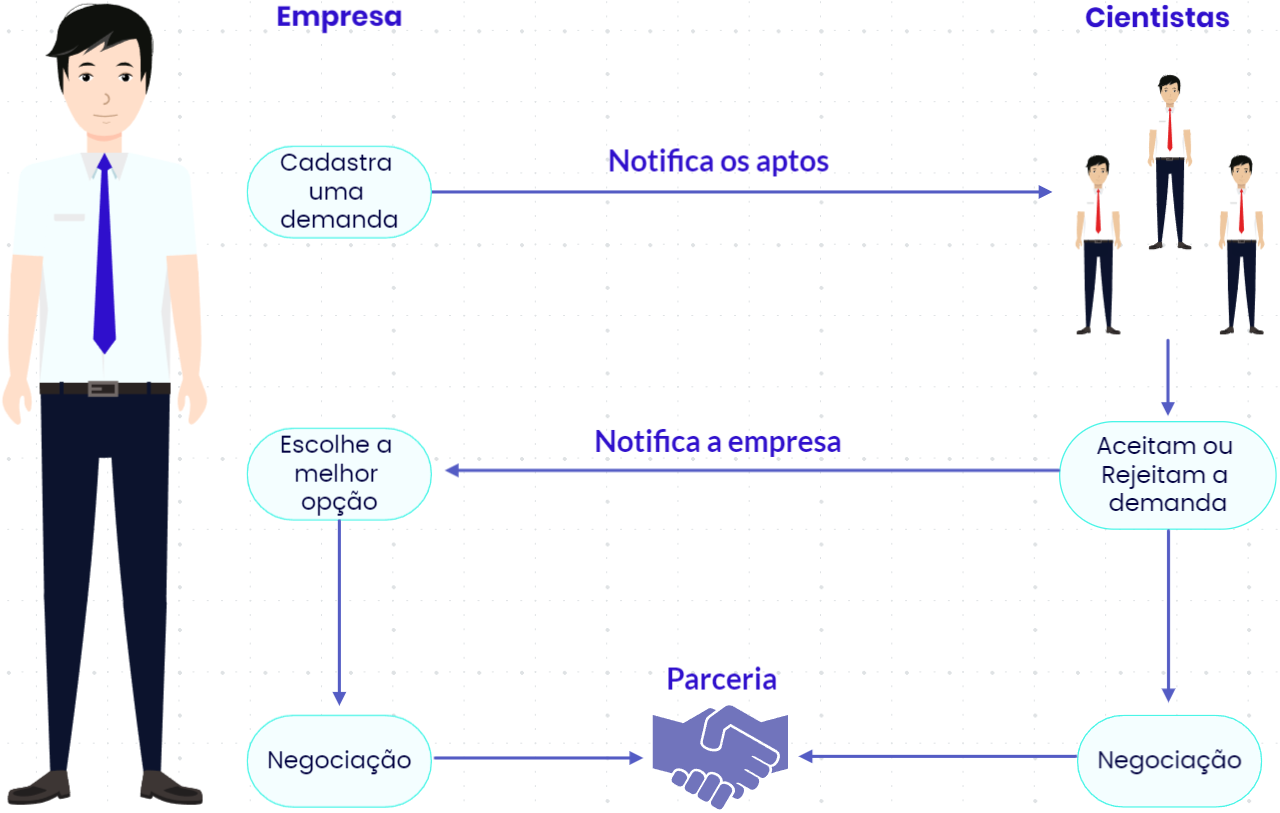
\includegraphics[width=\textwidth]{Flowchart.png}
    \fonte{Autoria Própria}
    \label{fig:fluxograma}
\end{figure}

\section{Análise e Validação}\label{sec:validacao}

Para corroborar o funcionamento e eficácia do projeto proposto, o \gls{direc}, responsável pela formação de parcerias entre empresas e a \gls{utfpr} irá validar a plataforma em conjunto com empresas já parceiras e membros do corpo acadêmico que aceitem participar do processo de validação e possam disponibilizar dados relacionados as experiências passadas na formação de parcerias. Também poderão ser comparados os resultados com outras ferramentas de busca de capital intelectual como, por exemplo, o \textit{LinkedIn}, \textit{Escavador} e a própria plataforma \textit{Lattes}, podendo-se utilizar de métricas que se julguem necessárias, como o tempo entre a criação de uma demanda e a formação de um parceria para atendê-lá.